\chapter{Clustering}\label{ch:clustering}

\section{Concetti generali}\label{sec:clu-concetti}
Il \textbf{clustering} raggruppa oggetti in \emph{cluster} tali che i punti nello stesso cluster siano tra loro simili, mentre punti in cluster diversi siano dissimili. È un compito \emph{unsupervised}: non si conoscono etichette a priori. La \emph{classificazione} è invece \emph{supervised} e richiede classi note per l’addestramento.

\subsection{Spazi metrici e funzioni distanza}\label{subsec:metric-spaces}
Si assume uno \textbf{spazio metrico} $(\mathcal{S},D)$, con $D$ che soddisfa:
\[
\begin{aligned}
\text{\textbf{Non negatività}}\quad & D(x,y) \ge \,0 && \forall\, x,y \in S,\\
\text{\textbf{Simmetria}}\quad & D(x,y) = D(y,x) && \forall\, x,y \in S,\\
\text{\textbf{Disuguaglianza triangolare}}\quad & D(x,y)+D(y,z) \ge D(x,z) && \forall\, x,y,z \in S.
\end{aligned}
\]

\paragraph{Distanze in spazi euclidei.}
Siano $\mathbf{x}=(x_1,\dots,x_n)$ e $\mathbf{y}=(y_1,\dots,y_n)\in\mathbb{R}^n$.

\[
\textbf{Distanza euclidea:}\quad
D_2(\mathbf{x},\mathbf{y})=\sqrt{\sum_{i=1}^{n}(x_i-y_i)^2}
\]

\[
\textbf{Distanza di Manhattan:}\quad
D_1(\mathbf{x},\mathbf{y})=\sum_{i=1}^{n}\lvert x_i-y_i\rvert
\]

\[
\textbf{Norma }L_r:\quad
D_r(\mathbf{x},\mathbf{y})=\Bigg(\sum_{i=1}^{n}\lvert x_i-y_i\rvert^{\,r}\Bigg)^{\!1/r},\ \ r\ge 1
\]

\[
\textbf{Norma }L_{\infty}:\quad
D_{\infty}(\mathbf{x},\mathbf{y})=\max_{1\le i\le n}\lvert x_i-y_i\rvert
\]

\[
\textbf{Distanza del coseno (angolare):}\quad
D_{\angle}(\mathbf{x},\mathbf{y})
=\arccos\!\left(
\frac{\sum_{i=1}^{n} x_i y_i}{\sqrt{\sum_{i=1}^{n} x_i^{2}}\ \sqrt{\sum_{i=1}^{n} y_i^{2}}}
\right),
\qquad \mathbf{x}\neq\mathbf{0},\ \mathbf{y}\neq\mathbf{0}.
\]



\paragraph{Spazi non euclidei.}
Per oggetti-insiemi o stringhe il centroide può non avere senso: si usa il \textbf{medoide} (elemento del dataset che minimizza la somma delle distanze agli altri).
Esempi di metriche:
\[
D_\mathrm{Jac}(S,T)=1- \frac{|S\cap T|}{|S\cup T|}\quad\text{(Jaccard)},
\]
Altri esempi di distanze sono:
\begin{enumerate}
  \item \textbf{Distanza di Edit}: il minimo numero di operazioni di cancellazione o inserzioni di caratteri da effettuare partendo da una stringa A per ottenere la stringa B. (es. A = abcde, B = acfdeg $\Rightarrow$ D(A, B) = 3).
  \item \textbf{Distanza di Hamming}: dati A, B vettori, il numero di componeneti in corrispondenza delle quali differiscono (es. A = (1, 0, 1, 0, 1), B = (1, 1, 1, 1, 0) $\Rightarrow$ D(A, B) = 3).
\end{enumerate}

\subsection{Tassonomia degli algoritmi}\label{subsec:taxonomy}
Tre famiglie principali:

\begin{enumerate}
  \item \textbf{gerarchici} (agglomerativi/divisivi);
  \item \textbf{partizionali} (es.\ k-means);
  \item \textbf{a densità} (DBSCAN/OPTICS/HDBSCAN).
\end{enumerate}

\paragraph{Bontà di un algoritmo.}
Dipende da: \emph{scalabilità}, supporto a attributi eterogenei, capacità di cogliere \emph{forme diverse} di cluster, \emph{robustezza} a outlier/rumore e dati mancanti, \emph{stabilità} all’aggiunta di nuovi dati, e \emph{interpretabilità} dei risultati. La scelta pratica è un compromesso tra qualità e costi computazionali.

\subsection{Alta dimensionalità: equidistanza e ortogonalità}\label{subsec:curse}
Spazi euclidei ad elevata dimensionalità soffrono del \emph{problema della dimensionalità}:
\begin{itemize}
  \item quasi tutte le coppie di punti risultano \textbf{equidistanti} e lontane tra loro;
  \item quasi tutte le coppie di vettori sono quasi \textbf{ortogonali}.
\end{itemize}

\paragraph{Equidistanza dei punti.}
Sia $D(\mathbf{x},\mathbf{y})=\|\mathbf{x}-\mathbf{y}\|_2$ con $\mathbf{x},\mathbf{y}\in[0,1]^n$ indipendenti.
Quando $n$ è grande, con alta probabilità:
\[
\underbrace{1}_{\text{limite inferiore}} \ \lesssim\ D(\mathbf{x},\mathbf{y})\ \lesssim\ \underbrace{\sqrt{n}}_{\text{limite superiore}}
\]
e \emph{solo una frazione trascurabile} di coppie è vicina ai due limiti. La \textbf{maggior parte} delle coppie ha una distanza
vicina alla media, circa $\sqrt{n}/3$ (concentrazione della distanza). Inoltre i prodotti scalari tendono a $0$,
così gli angoli sono prossimi a $90^\circ$ (quasi ortogonalità).

\paragraph{Conseguenze pratiche.}
Distinguerre “vicini” da “lontani” diventa difficile; conviene standardizzare le feature, ridurre la dimensionalità (es.\ PCA)
o usare metriche più adatte (cosine/angolare), soprattutto in presenza di dati sparsi.


\section{Clustering gerarchico}\label{sec:hierarchical}
\paragraph{Schema agglomerativo.}
(a) inizializza: ogni punto è un cluster; (b) ripeti: fonde i due cluster più vicini secondo una \emph{distanza tra cluster}; (c) termina con un criterio (numero desiderato di cluster o qualità).

\subsection{Distanza tra cluster (\emph{linkage})}\label{subsec:linkages}

\begin{figure}[htbp]
\centering
\begin{minipage}[t]{0.65\textwidth}
\vspace{0pt}
\begin{itemize}[leftmargin=1.2em]
  \item \textbf{Single-link}: $\min\{D(x,y): x\in C_i,\ y\in C_j\}$ (tende a catene).
  \item \textbf{Complete-link}: $\max\{D(x,y): x\in C_i,\ y\in C_j\}$ (favorisce cluster compatti).
  \item \textbf{Average-link}: media delle distanze su tutte le coppie $x\in C_i,\,y\in C_j$ (compromesso).
  \item \textbf{Centroid/medoid}: distanza tra centroidi (euclideo) o tra medoidi (generale).
\end{itemize}
\end{minipage}\hfill
\begin{minipage}[t]{0.27\textwidth}
\vspace{0pt}
\centering
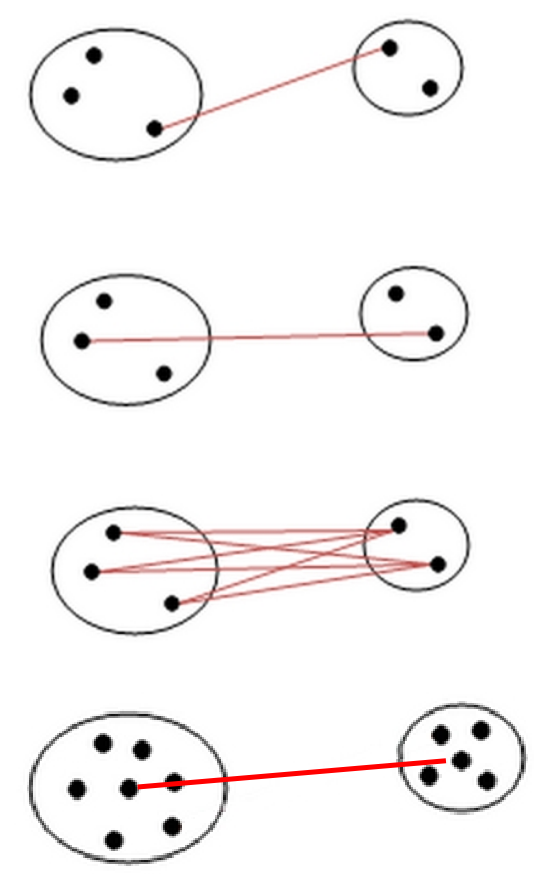
\includegraphics[width=\linewidth]{images/cluster_distances.png}
\caption{Esempi grafici delle diverse nozioni di distanza tra cluster.}
\label{fig:cluster_distances}
\end{minipage}
\end{figure}

\subsection{Dendrogramma e criteri di stop}\label{subsec:dendro}
Il \textbf{dendrogramma} registra le fusioni; tagliandolo a una certa altezza si ottiene la partizione.
Criteri di terminazione:
(i) fermarsi a $k$ cluster prefissati;
(ii) fermarsi quando l’unione successiva degrada troppo la qualità (es.\ aumento del diametro o della distanza media intra-cluster).

\begin{figure}
  \centering
  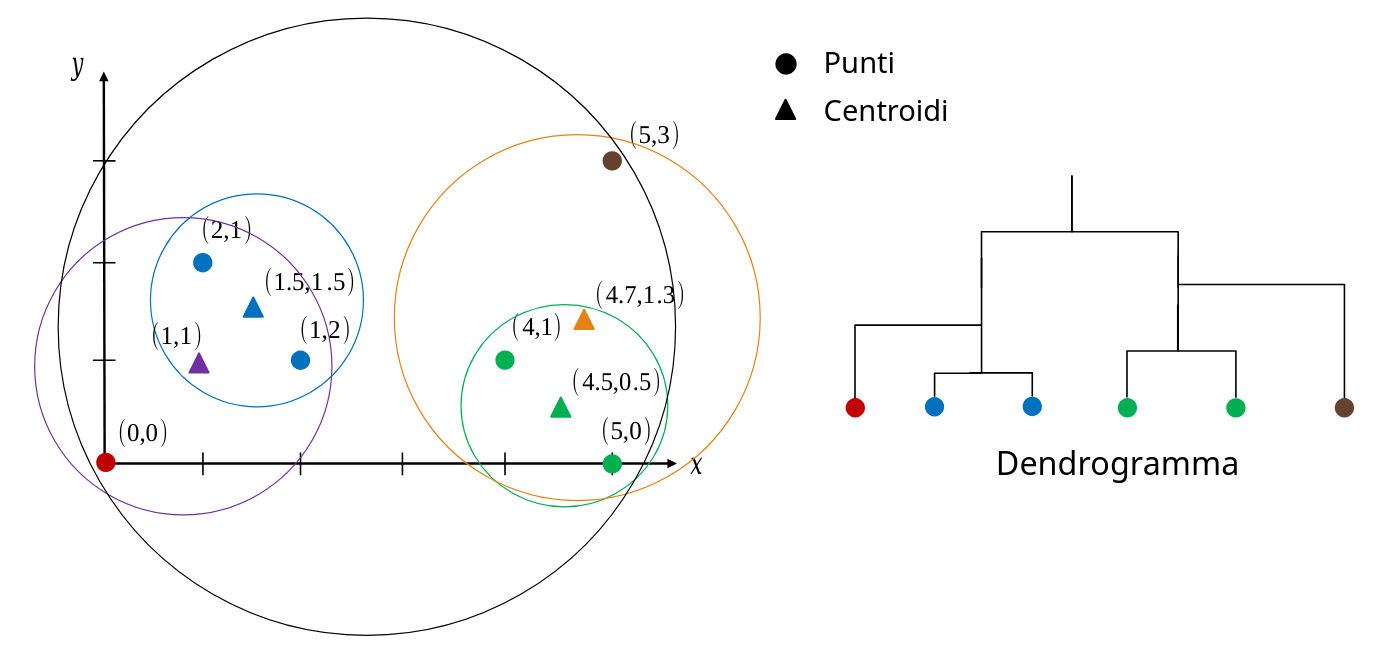
\includegraphics[width=\textwidth]{images/dendograms.png}
  \caption{A sinistra: punti nel piano con centroidi (triangoli) e cerchi che schematizzano la coesione dei gruppi; i colori indicano i cluster. A destra: dendrogramma agglomerativo che mostra l’ordine di fusione e l’altezza (distanza di linkage). Un taglio orizzontale del dendrogramma determina il numero di cluster.}
  \label{fig:dendograms}
\end{figure}

\subsection{Altri criteri di combinazione}\label{subsec:altri-criteri}
Si può fondere la coppia che massimizza la \emph{qualità} del cluster risultante.
Definizioni utili: \emph{raggio} $=\max_{x\in C} D(x,\mathrm{centroide}(C))$; \emph{diametro} $=\max_{x,y\in C} D(x,y)$.

\subsection{Versioni divisive}\label{subsec:divisive}
Approccio \textbf{top–down}: un'altra versione dove si parte da un unico cluster e lo si \emph{divide} iterativamente scegliendo il miglior \emph{taglio}. Le stesse metriche di distanza/qualità si applicano in modo duale.

\subsection{Complessità e ottimizzazioni}\label{subsec:hclust-compl}

\paragraph{Analisi \emph{naive}.}
Al primo passo si valuta la distanza per ogni coppia di cluster e si sceglie la migliore: costo $\Theta(n^2)$.
Dopo ogni fusione i cluster diminuiscono di uno, quindi i passi successivi costano, nell’ordine,
$(n-1)^2,(n-2)^2,\dots,2^2$.
\[
T_{\text{naive}}
=\sum_{k=2}^{n} k^{2}
=\frac{n(n+1)(2n+1)}{6}-1
=\Theta(n^{3}).
\]
(Spazio tipico: matrice delle distanze $O(n^2)$.)

\paragraph{Ottimizzazione con \emph{coda di priorità}.}
Usando una coda di priorità (min-heap) sulle distanze tra cluster:
\begin{itemize}
  \item accesso al minimo (\emph{peek}) in $O(1)$; inserimenti e cancellazioni in $O(\log n)$;
  \item ad ogni fusione si \emph{rimuovono} al più $2(n-1)$ distanze (quelle dai due cluster che si fondono): $O(n\log n)$;
  \item si \emph{calcolano e inseriscono} le distanze tra il nuovo cluster e gli altri (al più $n-2$): $O(n\log n)$.
\end{itemize}
Su $n-1$ fusioni:
\[
T_{\text{heap}}=O\big(n \cdot (n\log n)\big)=O(n^{2}\log n).
\]
Risultato: la complessità scende da $O(n^{3})$ a circa $O(n^{2}\log n)$ mantenendo la matrice (o la coda) aggiornata a ogni iterazione.


\section{Clustering partizionale: k-means}\label{sec:kmeans}
Metodi per spazi euclidei che partizionano i dati in $k$ cluster minimizzando la somma delle distanze al quadrato dai centroidi.

\subsection{Algoritmo base}\label{subsec:kmeans-basic}
\begin{enumerate}
  \item \textbf{Inizializza} $k$ centroidi (idealmente separati).
  \item \textbf{Assegna} ogni punto al centroide più vicino (distanza euclidea).
  \item \textbf{Aggiorna} ogni centroide come media dei punti assegnati.
  \item \textbf{Ripeti} finché i centroidi si stabilizzano o il miglioramento è sotto soglia.
\end{enumerate}
Converge in pochi round, ma solo a un ottimo \emph{locale}.

\subsection{Inizializzazione}\label{subsec:init}
Scelta \emph{greedy}:
\begin{enumerate}
  \item Si sceglie il primo punto in maniera casuale o lo si aggiunge all'insieme $S$ dei punti già selezionati, inizialmente vuoto.
  \item Si calcola la massima distanza minima dai centroidi scelti.
  \item Si ripete il passo 2. finché $|s| < k$.
\end{enumerate}

\begin{figure}[htpb]
  \centering
  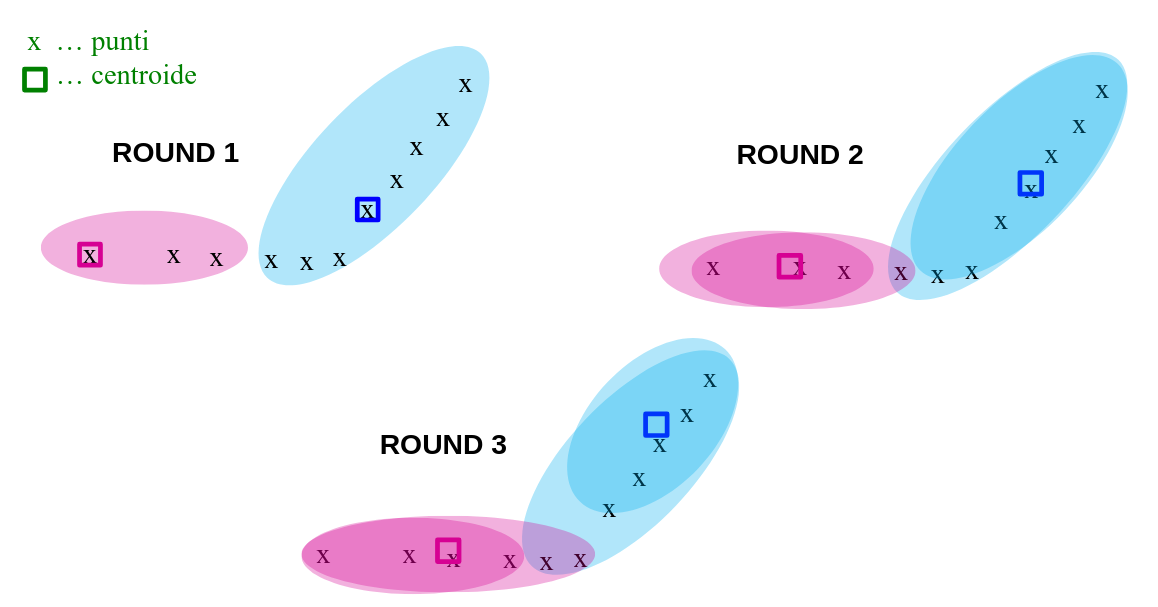
\includegraphics[width=0.7\textwidth]{images/k-means.png}
  \caption{K-means: evoluzione in tre round. 
  Round 1: inizializzazione e prime assegnazioni ai centroidi (quadrati). 
  Round 2: ricalcolo dei centroidi e riassegnazione dei punti (X). 
  Round 3: i centroidi si stabilizzano e i cluster (ellissi colorate) convergono.}
  \label{fig:k-means-example}
\end{figure}

\subsection{Funzione obiettivo e arresto}\label{subsec:objective}
Con partizione $C_1,\dots,C_k$ e centroidi $\mu_r$:
\[
J=\sum_{r=1}^k \sum_{x\in C_r} \|\mathbf{x}-\mu_r\|_2^2.
\]
Arresto quando $\Delta J$ tra iterazioni consecutive è sotto soglia o quando non cambia l’assegnazione. Con metriche diverse da euclidea il centroide non è il minimizzatore naturale.

\subsection{Scelta del numero di cluster $k$}\label{subsec:scelta-k}
Poiché $k$ non è noto a priori, si esegue il metodo per più valori e si seleziona quello che ottimizza una metrica di qualità interna.

\paragraph{Funzione obiettivo.}
Per $k$ cluster $C_1,\dots,C_k$ con centroidi $\mathbf{c}_1,\dots,\mathbf{c}_k$, la funzione standard è
\[
W(k)=\sum_{i=1}^k \sum_{\mathbf{x}\in C_i}\|\mathbf{x}-\mathbf{c}_i\|_2^2,\qquad 
\bar W(k)=\frac{W(k)}{n}\;\;(\text{distanza media al centroide}).
\]
$W(k)$ è decrescente in $k$.

\begin{figure}[htbp]
  \centering
  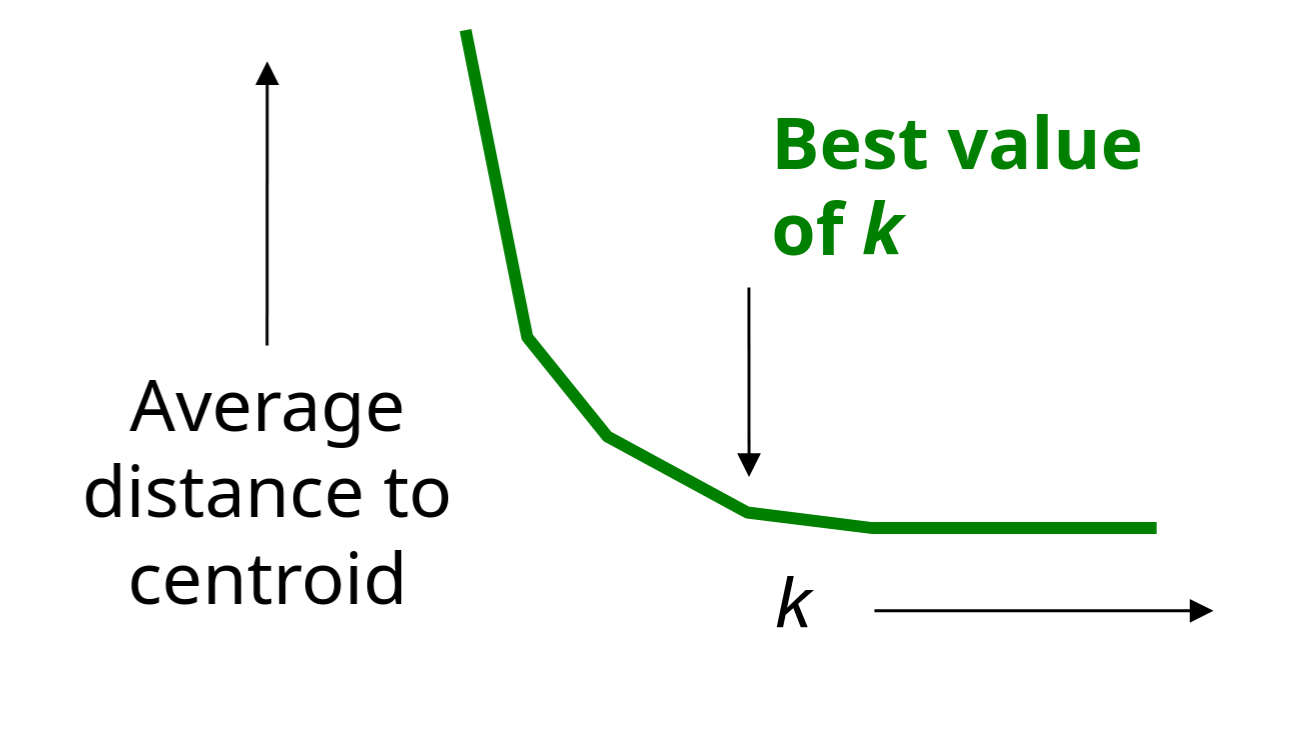
\includegraphics[width=0.8\textwidth]{images/elbow-k.png}
  \caption{Metodo (\emph{elbow}). Si traccia la distanza media dal centroide (o WCSS/n) al variare di $k$; il valore “ottimo” è nel punto di flesso, dove l’aumento di $k$ porta benefici marginali trascurabili.}
  \label{fig:elbow}
\end{figure}

\paragraph{Metodo \emph{elbow}.}
Si calcola $\bar W(k)$ per $k=k_{\min},\dots,k_{\max}$ e si sceglie il $k$ per cui il calo di $\bar W$ passa da “ripido” a “lento” (punto di flesso).
\begin{itemize}
  \item \emph{Procedura pratica:} si valuta $\bar W(k)$ su una griglia di valori e si ispeziona il grafico $\bar W$ vs $k$.
  \item \emph{Variante a ricerca binaria:} fissati due estremi $x<y$, si prende $z=\lfloor(x+y)/2\rfloor$, si calcola $\bar W(z)$ e si sostituisce l’estremo \emph{più vicino} a $\bar W(z)$ con $z$; si ripete finché l’intervallo è piccolo. Il $k$ finale approssima il gomito.
\end{itemize}
\emph{Nota:} se la curva non mostra un gomito netto, l’elbow diventa ambiguo e conviene affiancarlo a silhouette/stabilità.



\paragraph{Metodo \emph{silhouette}.}
Per ogni punto $\mathbf{x}$ assegnato al cluster $C_i$:
\[
a(\mathbf{x})=\frac{1}{|C_i|-1}\sum_{\mathbf{y}\in C_i,\ \mathbf{y}\neq \mathbf{x}}\!\!\!\!\|\mathbf{x}-\mathbf{y}\|, \qquad
b(\mathbf{x})=\min_{j\neq i}\ \frac{1}{|C_j|}\sum_{\mathbf{y}\in C_j}\|\mathbf{x}-\mathbf{y}\|.
\]
Lo \emph{score di silhouette} del punto è
\[
s(\mathbf{x})=\frac{b(\mathbf{x})-a(\mathbf{x})}{\max\{a(\mathbf{x}),\,b(\mathbf{x})\}}\in[-1,1].
\]
Valori vicini a $1$ indicano assegnazioni “pulite”, vicini a $0$ punti al confine, negativi assegnazioni sbagliate. Si sceglie
\[
k^\star=\arg\max_k\ \frac{1}{n}\sum_{r=1}^n s(\mathbf{x}_r).
\]
\emph{Regole d’uso.} Calcolare gli indici su più esecuzioni (inizializzazioni diverse) e riportare media/deviazione; standardizzare le feature prima del confronto; evitare $k$ troppo grandi che trivialiscono $\bar W$ ma peggiorano la silhouette.

% --------------------------------------------------------------------

\subsection{Complessità computazionale}\label{subsec:kmeans-compl}
Ogni iterazione del \emph{k}-means ha due passi:
\begin{enumerate}
  \item \textbf{Assegnamento} (nearest–centroid): per ciascun punto si valuta la distanza verso i $k$ centroidi. Costo $O(nkd)$ in $\mathbb{R}^d$ (spesso si sottintende $d$, scrivendo $O(nk)$).
  \item \textbf{Aggiornamento dei centroidi}: si ricalcolano le medie dei cluster. Costo $O(nd)$.
\end{enumerate}
Con $t$ iterazioni totali:
\[
T(n,k,d,t)=O(t\,n\,k\,d)\quad\text{(nelle slide: }O(tkn)\text{)}.
\]
